%%%%%%%%%%%%
%
% $Beschreibung: Sicherheitshinweise zum Demonstrator $
% $Autor: Theilmann $
% $Datum: 02.05.2024 $
% $Pfad: SafetyGuidelines.tex $
% $Version: 1 $
%
%%%%%%%%%%%%

\chapter{Sicherheitshinweise}


\textbf{Seien Sie bitte sehr vorsichtig bei jeder Interaktion mit dem Demonstrator. Bei diesesm Demonstrator handelt es sich um ein elektrisches Gerät mit beweglichen Teilen}:


	\begin{enumerate} 
		\item Das Gerät ist nur für den Innenbereich bestimmt. Setzen Sie den Demonstrator keiner Feuchtigkeit aus. Halten Sie den Demonstrator in einer trockenen Umgebung in einem Mindestabstand von 30\ cm zu anderen Gegenständen.
		
		\item Stellen Sie den Demonstrator immer an einem stabilen Ort auf, sodass er nicht herunterfallen oder umkippen kann.	
		
	\begin{figure}[h]
		\centering
		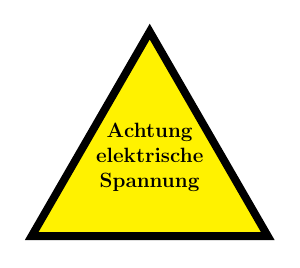
\begin{tikzpicture}[scale=0.3,transform shape]
				
				% Dreieck mit Schwarzem Rand
				\fill[yellow] (0,0) -- (5,8.66) -- (10,0) -- cycle;
				\draw[line width=1mm, black] (0,0) -- (5,8.66) -- (10,0) -- cycle;
									
				% Text
				\node[align=center] at (5,4.2) {\\\\\\\\\\\Huge\textbf{Achtung}\\\\\Huge\textbf{elektrische}\\\\\Huge\textbf{Spannung}};
				
			\end{tikzpicture}
		\end{figure}
			
			 	\item Die Stromversorgung des Demonstrators erfolgt über eine Steckdose 230\ V. Schließen Sie den Demonstrator niemals an ein anderes Netzteil an, da dies zu Fehlfunktionen oder Beschädigungen des Demonstrators führen kann. 
				
				\item Verlegen Sie das Netzkabel so, dass Sie nicht darüber stolpern, darauf treten oder anderweitig Schaden nehmen können. Vergewissern Sie sich, dass das Netzkabel nicht mechanisch oder anderweitig beschädigt ist.
				 
				\item Wenn Sie das Netzkabel aus der Steckdose ziehen, so sollten Sie direkt an dem Stecker ziehen und nicht am Netzkabel, um das Risiko einer Beschädigung des Steckers oder der Netzsteckdose zu verringern.
												
				\item Nehmen Sie niemals das Netzteil des Demonstrators auseinander, alle Reparaturen müssen von einem qualifizierten Techniker durchgeführt werden.
				
				\begin{figure}[h]
					\centering
					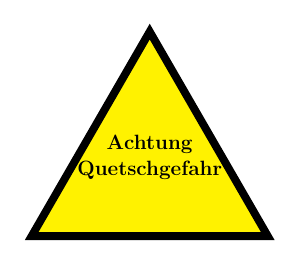
\begin{tikzpicture}[scale=0.3,transform shape]
						
						% Dreieck mit Schwarzem Rand
						\fill[yellow] (0,0) -- (5,8.66) -- (10,0) -- cycle;
						\draw[line width=1mm, black] (0,0) -- (5,8.66) -- (10,0) -- cycle;
						
						% Text
						\node[align=center] at (5,4.2) {\\\\\\\\\\\Huge\textbf{Achtung}\\\\\Huge\textbf{Quetschgefahr}};
						
					\end{tikzpicture}
				\end{figure}
				
				\item Greifen Sie nicht in das Innere des Demonstrators, während er noch im Betrieb ist. Eine Verletzung kann durch die beweglichen Teile verursacht werden.
				
				\item Verhindern Sie, dass Kinder unbeaufsichtigt auf den Demonstrator zugreifen können, auch wenn dieser nicht im Betrieb ist. 
				
				\item Lassen Sie den Demonstrator nicht unbeaufsichtigt, solange er noch im Betrieb ist.	
	\end{enumerate}
